\documentclass{article}
\usepackage[T1]{fontenc}
\usepackage{lmodern}
\usepackage{graphicx}
\usepackage{amsmath,amssymb}
\usepackage[a4paper,margin=2cm]{geometry}
\usepackage[absolute,overlay]{textpos}
\setlength{\TPHorizModule}{1mm}
\setlength{\TPVertModule}{1mm}
\usepackage[indonesian]{babel}
\usepackage{hyperref}
\setlength{\emergencystretch}{2em}
% unit: Halaman 21

\begin{document}

% === Halaman 21 (llm) ===

\vspace{273.24mm}

\begin{itemize}
  \item[] \textcolor{red}{\textbf{for} $i \gets 1$ \textbf{to} $r$ \textbf{do}\
  \textcolor{red}{$A \gets ((A \oplus B) \lll B) + S[2i]$}\
  \textcolor{red}{$B \gets ((B \oplus A) \lll A) + S[2i+1]$}\
  \textcolor{red}{\textbf{endfor}}
\end{itemize}

\vspace{20mm}

Cipherteks pada putaran terakhir disimpan di dalam $A$ dan $B$.

Gabungan keduanya adalah blok cipherteks yang berukuran 64 bit.

\vspace{10mm}

Proses enkripsi satu putaran:

% deskripsi: Diagram alur proses enkripsi satu putaran yang menunjukkan operasi XOR, rotasi bit (<<<), dan penjumlahan dengan konstanta S, menghasilkan output A_i dan B_i dari input A_{i-1} dan B_{i-1}.
% bbox normalisasi: [0.5600, 0.0000, 0.8400, 0.9200]
\begin{textblock*}{58.80mm}(117.60mm,0.00mm)
\noindent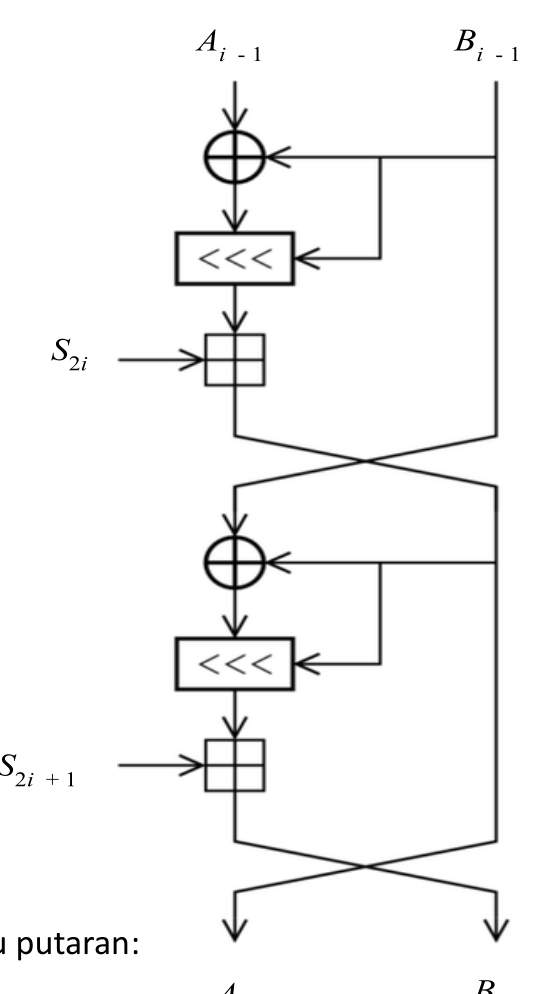
\includegraphics[width=58.80mm,height=273.24mm]{../../images/llm/page_021_img_01.png}%
\end{textblock*}

\end{document}
